\documentclass[a4,12pt]{article}
\usepackage[utf8]{inputenc}
\usepackage[spanish]{babel}
\usepackage[margin=2cm]{geometry}
\usepackage{graphicx}
\usepackage{import}
\usepackage{color}
\usepackage{times}
\usepackage{listings}

\renewcommand{\familydefault}{\sfdefault}


\usepackage{hyperref}

\hypersetup{
    pdfborder = {0 0 0}
}

\title{Cálculo del tiempo del algoritmo de ordenación QuickSort para diferentes tamaños de problema}

\author{Lydia Martínez-Fortún Martínez}



\begin{document}

\maketitle



\begin{abstract}
En este documento en \LaTeX{} se explica el calculo del algoritmo de ordenación QuickSort hecho en Octave y los tiempos de ejecución para diferentes tamaños de problemas.
\end{abstract}

\tableofcontents

\newpage

\section{Introducción al algoritmo}

En este documento se muestra como hacer un algoritmo de ordenación en Octave. En este caso he implementado el algoritmo QuickSort, que lo que hace es elegir un pivote y dividiendo el vector en los mayores, menores o iguales a él.



\section{QuickSort}

El algortimo Quick Sort esta basado en la técnica de divide y vencerás, el cual permite en ordenar n elementos en un tiempo proporcional a \emph{n log n}. El algoritmo elige un elemento de la lista al que se le llama pivote. Despues el algoritmo separa en tres vectores los menores, los mayores, y los iguales al pivote. En este momento se van haciendo llamadas recurisivas, de estas listas hasta que sean de tamaño uno. Al final se combinan y da como resultado el vector original ordenado.


\subsection{Pseudocódigo}
\lstset{language=Pascal}
\begin{lstlisting}[frame=single][language=Octave]
FUNCION QuickSort(vector)
	SI logitud(vector)>1  ENTONCES
		//Se elige de pivote el elemento central 
		del vector
		Pivote = vector(posicionCentral)
		PARA cada elemento n de vector
			SI n < Pivote ENTONCES
				insertar a la lista menores
			FINSI
			SI n = Pivote ENTONCES
				insertar a la lista iguales
			FINSI
			SI n > Pivote ENTONCES
				insertar a la lista mayores
			FINSI
		FINPARA
		VectorOrdenado =Concatenar(QuickSort(menores), 
					QuickSort(iguales), 
					QuickSort(mayores))	
	Devolver VectorOrdenado	
	FINSI
FINFUNCION

\end{lstlisting}

\subsection{Código en Octave}
\subsubsection{Funcion QuickSort en Octave}
Para la implementacion de la función QuickSort he hecho de funciones de octave. Una de ellas es la funcion \emph{round} que redondea el valor obtenido de la division. Otra función que he usado es \emph{find}, dada una condición crea un vector con los valores que la cumplan, en el primer caso crea un vector con los valores menores que el pivote.
\bigskip %para separa el texto del codigo
\lstset{language=Octave}
\begin{lstlisting}[frame=single][language=Octave]
function vectorOrdenado=quickSort(v)     
  vectorOrdenado = v;
  n=length(v);
  if(n > 1)          
     pivote=v(round(n/2)+1);             
     menores = find(vectorOrdenado < pivote); 
     iguales = find(vectorOrdenado == pivote);
     mayores=find(vectorOrdenado > pivote);
     vectorOrdenado  = [quickSort(vectorOrdenado(menores));
     			vectorOrdenado(iguales); 
     			quickSort(vectorOrdenado(mayores))];
  end
endfunction
\end{lstlisting}
\subsubsection{Funcion para calcular los tiempos de ejecucion de Quick Sort}
Este algoritmo calcula el tiempo de ejecución de la función Quick Sort desde tamaño 1 hasta el tamaño máximo pasado por parametro \emph {tamMax}. Para calcular el tiempo de ejecución he usado las funciones tic y toc de Octave. En toc se guarda el tiempo, y este lo almaceno en un vector \emph{tiemposTam}, el cual cada indice corresponde al tamaño del vector ejecutado.
La función \emph{zeros(1,0)} crea un vector de una fila y lo rellena con ceros.
Para que los casos a probar sean los mas dispares posibles he usado la funcion \emph{rand(tam,1)} para que los valores de los vectores sean aleatorios. La función \emph{rand} devuelve numeros aleatorios entre cero y uno. Debido a esto la multiplico por 2000, para que el rango de valores sea aun mas amplio.
\bigskip %para separa el texto del codigo
\lstset{language=Octave}
\begin{lstlisting}[frame=single][language=Octave]
function tiemposTam=tiempoQuickSort(maxTam)
	tiemposTam=zeros(1,0);
	tam=1;
	while(tam<=maxTam)
		vector=(rand(tam,1)*500);	
		tic,u=quickSort(vector); 
		tiemposTam(tam)=toc;
		if(length(vector)==20)
			disp(El vector inicial es el siguiente: );
			printf( %f ,vector);
			printf("\n");
			
			\end{lstlisting}
			\begin{lstlisting}[frame=single][language=Octave]
			
			disp(El vector ordenado es el siguiente: );
			printf( %f ,u);
			printf("\n");
		end
		tam=tam+1;
		endwhile

endfunction
\end{lstlisting}
\subsubsection{Codigo para usar de las funciones}
Con este codigo se obtienen las graficas. El el primer caso se obtiene una grafica de los tiempos de ejecucion de vectores de tamaño 1 hasta 20. En el segundo caso se ejecuta tres veces con tamaño del vector igual a 500 el algoritmo  para obtener valores más precisos haciendo un promedio
Para obteneer las graficas he usado la función plot de octave.
\bigskip %para separa el texto del codigo
\lstset{language=Octave}
\begin{lstlisting}[frame=single][language=Octave]

tiempos20=tiempoQuickSort(20);
plot(tiempos20,'m--');
title (Tiempo de ejecucion de QuickSort);
xlabel (Tam. del vector);
ylabel (Tiempo);
print -dpng Grafica20.png 

tiempos500_1=tiempoQuickSort(500);
tiempos500_2=tiempoQuickSort(500);
tiempos500_3=tiempoQuickSort(500);
plot(tiempos500_1,'m', tiempos500_2,'r--',tiempos500_3,'c+');
title (Tiempo de ejecucion de QuickSort);
xlabel (Tam. del vector);
ylabel (Tiempo);
print -dpng Grafica500.png 
\end{lstlisting}
\newpage
\section{Resultados obtenidos}
Como ejemplo de resultado tamaño que sea apreciable, voy a mostrar los datos obtenidos de un vector de 20 elementos.
\subsection{Vector inicial obtenido aleatoriamente}
El vector que se ha obtenido es el que se muestra en la siguiente figura:
\begin{figure}[h]
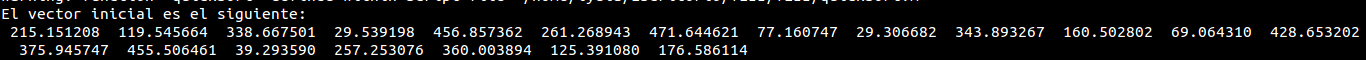
\includegraphics[width=1\textwidth]{Graficos/vectorInicial}
\caption{Vector Inicial}
\label{fig:vectorInicial}
\end{figure}

\subsection{Vector ordenado obtenido}
Como se puede observar en la figura es el mismo vector pero esta ordenado. 
El \textbf{tiempo de ejecución del algoritmo QuickSort es de 0.0015240}.
\begin{figure}[h]
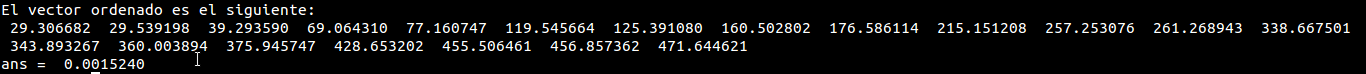
\includegraphics[width=1\textwidth]{Graficos/vectorOrdenado}
\caption{vector Ordenado}
\label{fig:vectorOrdenado}
\end{figure}

\section{Tiempos de ejecución}
A continuancion se muestran la gráficas obtenidas, la primera de ellas muestra el tiempo de ejecución para vectores de tamaño 1 hasta tamaño 20.
 
 \medskip
La segunda gráfica muestra tres lineas, corrrespondientes a tres pruebas, con vectores aleatorios partiendo igualmente de tamaño 1 y ahora llegando hasta tamaño 500.
 
 \medskip
Como se puede observar en las graficas siguientes el caso peor no tiene porque ser el que mas elementos tenga. De hecho el peor caso depende mayoritariamente del pivote  escogido. El peor caso se da cuando se el pivote elegido esta al extremo de la lista, este caso el orden de ejecución teoricamente es de $O(n^2)$.
El mejor caso, es cuando el pivote es el elemento centrar de la lista, y esta se divide en dos sublistas de igual tamaño. En el mejor caso el orden de ejecución teoricamente es de $O(nlogn)$. Ademas, en tiempo promedio teoricamente el algoritmo tambien tarda $O(nlogn)$.
\newpage
\subsection{Grafica de 1 a 20 elementos}
En la siguiente gráfica se muestran los tiempos de ejecucion para vectores de tamaño 1 hasta tamaño 20.

Como se puede observar, el tiempo no aumenta constantemente. Para el vector de tamaño 7 se obtiene un tiempo de ejecucion aproximado de 0.0015 el cual es mayor al tiempo de ejecución de tamaño 18. Esto puede deberse a que el pivote escogido por el de tamaño 7 estaba mas pegado a los extremos que el de tamaño 18, lo que hace que el tiempo de ejecución aumente.
\begin{figure}[h]
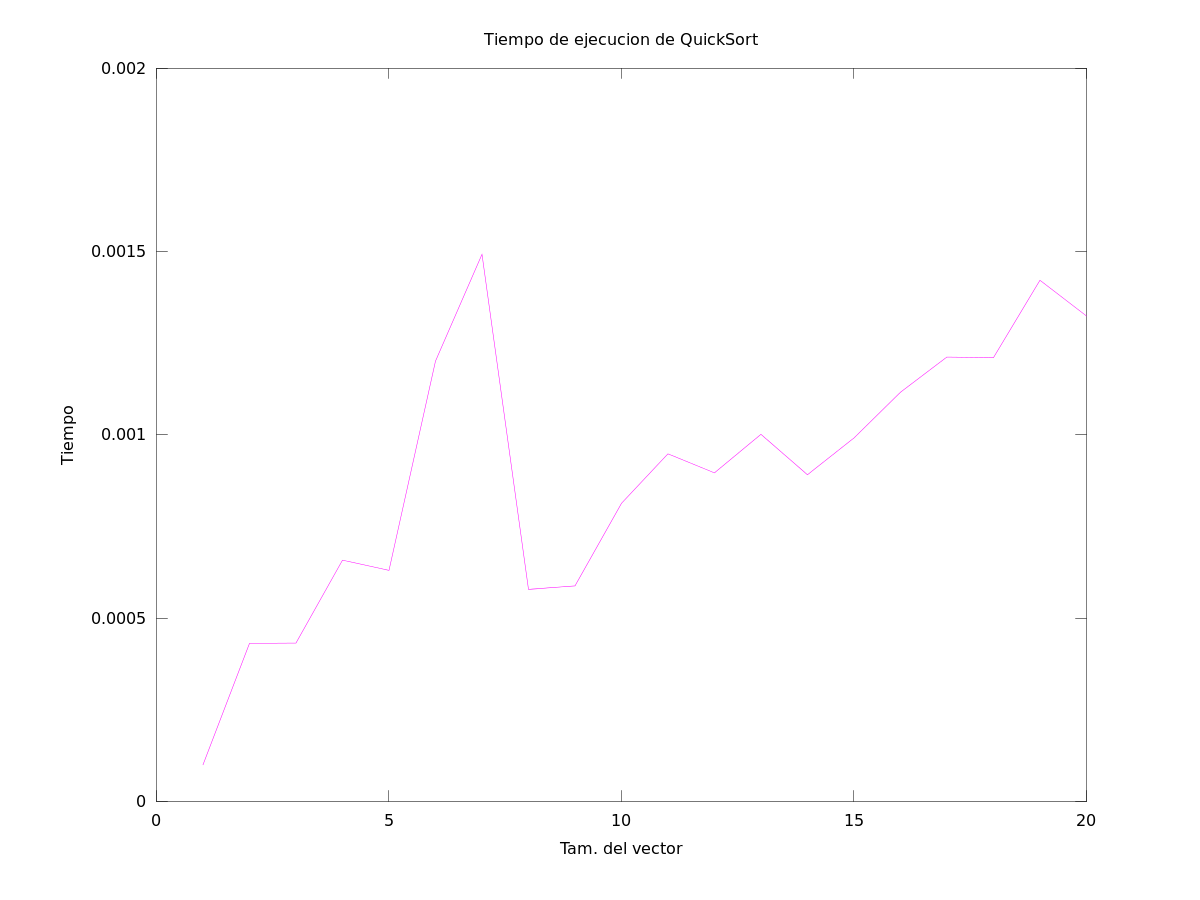
\includegraphics[width=1\textwidth]{Graficos/Grafica20}
\caption{Grafica de tiempos de ejecución 1 a 20 elementos}
\label{fig:Grafica20}
\end{figure}
\newpage
\subsection{Grafica de 1 a 500 elementos con tres pruebas}
En la siguiente gráfica se muestran el tiempo de ejecución de vectores de 1 a 500, con tres pruebas diferentes.

Como se observa en la figura, los tiempos aumentan conforme aumenta el tamaño del vector. 
\begin{figure}[h]
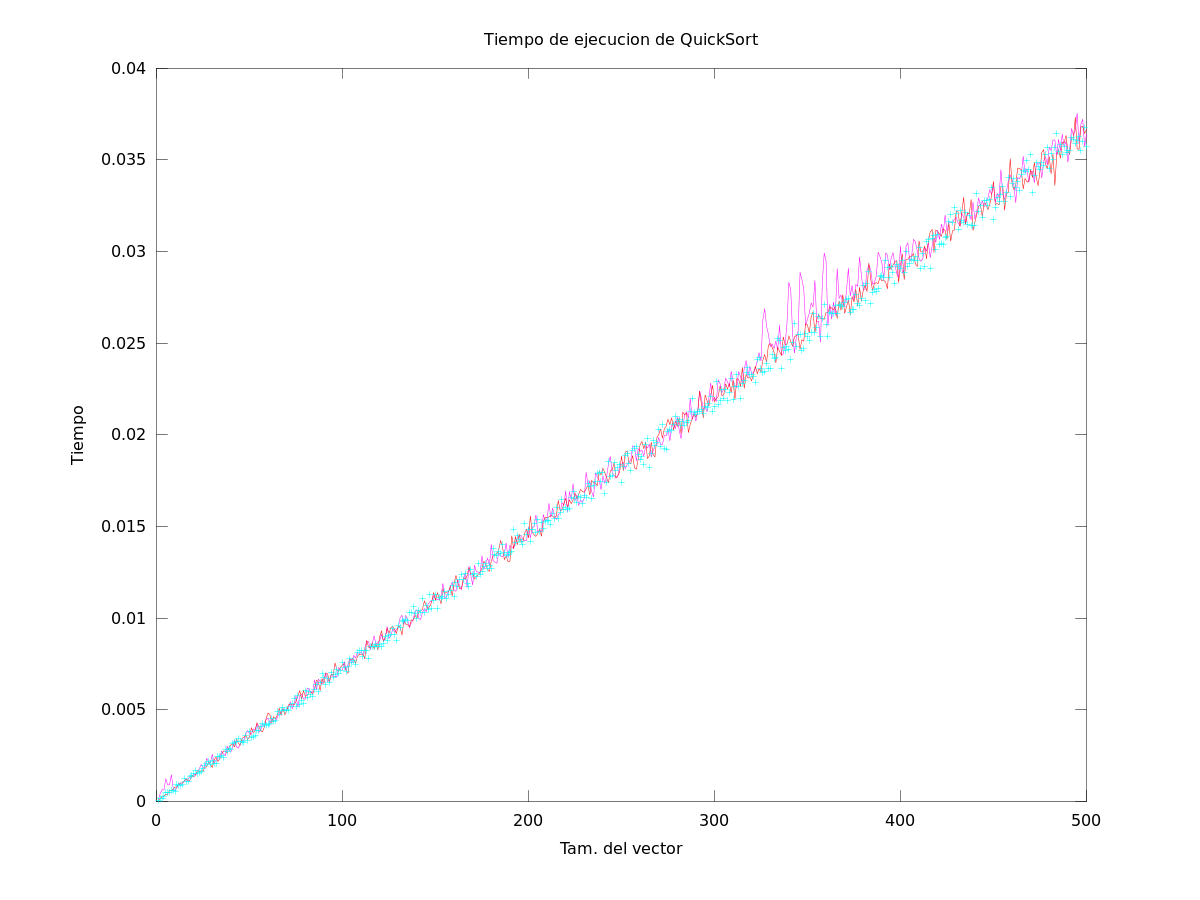
\includegraphics[width=1\textwidth]{Graficos/Grafica500}
\caption{Grafica de tiempos de ejecución 1 a 500 elementos con tres pruebas}
\label{fig:Grafica500}
\end{figure}
\subsection{Grafica de tiempos medios de ejecución}
En la siguiente gráfica se muestra el tiempo medio de ejecución, obtenido de las tres graficas anteriores.

En esta gráfica tambien se observa que el crecimiento es de orden similiar a lineal, mas proximo al mejor caso teorico de $O(nlogn)$, y a su vez es el orden promedio teorico del algoritmo que al peor caso que seria cuadratico $O(n^2)$.
\begin{figure}[h]
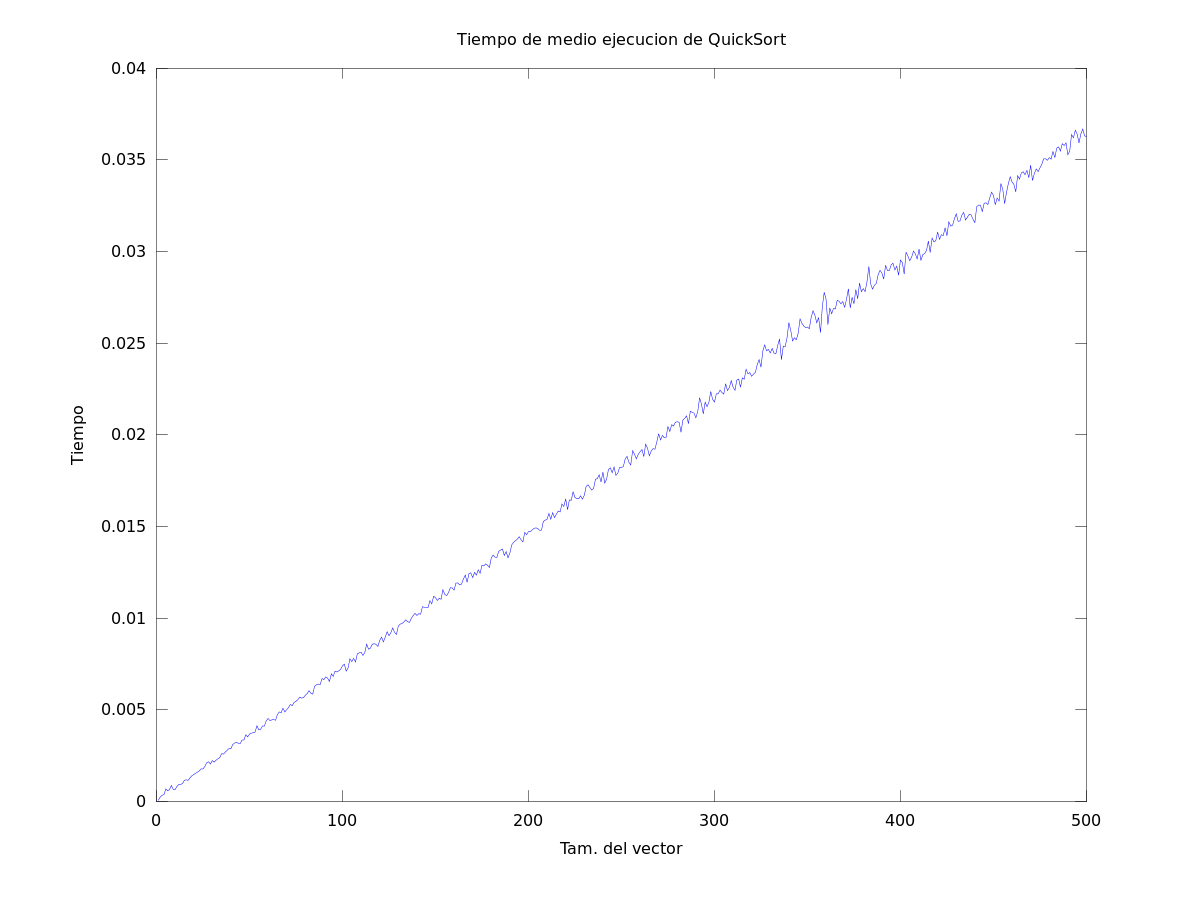
\includegraphics[width=1\textwidth]{Graficos/tiemposMedios}
\caption{Grafica de tiempos de medios ejecución 1 a 500 elementos}
\label{fig:tiemposMedios}
\end{figure}




\begin{thebibliography}{99}
\bibitem{WikiBooks} Latex:\\ \url{http://en.wikibooks.org/wiki/LaTeX/Floats,_Figures_and_Captions}
\bibitem{Wikipedia} Quick Sort:\\ \url{http://es.wikipedia.org/wiki/Quicksort}
\bibitem{fceia} Latex Espacios verticales: \\ \url{http://www.fceia.unr.edu.ar/lcc/cdrom/Instalaciones/LaTex/latex.html#SECTION02122000000000000000}
\bibitem{Niurka Rodriguez Quintero} Breve introducción al OCTAVE: \\ \url{http://euler.us.es/~niurka/clases/intro-niu.pdf}
\bibitem{github} GitHub: \\ \url{https://github.com}
\bibitem{wikibooks} Latex Basics: \\ \url{http://en.wikibooks.org/wiki/LaTeX/Basics}
\bibitem{rafalinux} Código en Latex: \\ \url{http://www.rafalinux.com/?p=599}

\end{thebibliography}

\end{document}

